\lstset{
frame=single,
language = {C++},
tabsize = 4,
captionpos=b,
showstringspaces=false,
numbers=left,
keywordstyle = \color{blue},
keywordstyle=[2]\color{gray},
stringstyle = \color[rgb]{0.64,0.08,0.08},
commentstyle = \color[rgb]{0,0.5,0},
numberstyle=\sffamily\tiny,
morecomment=[l]{\#}
%morekeywords={WORD, DWORD, PWORD, PDWORD, LPWORD, LPDWORD, QWORD, PQWORD,
%INT, INT32, INT64, UINT, UINT32, UINT64, LONG, LONGLONG, SHORT,},
}

%==============================================================================================================================
\chapter{Introduction}
\label{ch1}

Nowadays, many services allow their users to have their essential documents saved and safely backed up somewhere in the \textit{cloud}. Be it photos, videos, or just some notes saved in a Word\footnote{\url{https://www.microsoft.com/en-ww/microsoft-365/word}} document, today's technology allows anyone to access their files from any device. For example, imagine a typical browser-based could service. All that is required is for the user to have an internet connection and login, prove their identity to the \textit{server}, and the application on the user's device, the \textit{client}, takes care of the rest. After successful authentication, the user's files are available to read, download, and upload. Manually, these actions can become quite a bit of an overhead as the file count increases. What if the number of users that have access increases as well? 

The answer is - controlled access to remote documents and version control, which should be present on the server's side. In this thesis's case, the basis is an internal, non-formal API description of such a server, which will be referred to as The Validated Data Storage project (VDU). As such, this thesis analyzes previously mentioned requirements of the API access and creates a client-side application for Microsoft Widnows\footnote{\url{https://www.microsoft.com/en-us/windows}} from the ground up. To allow for a better user experience, this thesis showcases an implementation of a virtual file system, present on a virtual disk, integrated right into the desktop environment of Windows. This type of integration means being able to seamlessly view and or modify a file stored in the cloud, as if it was present on a virtual disk, without the need to download or upload after each modification constantly manually. 

WinFsp\cite{WinFsp} allows for implementing a filesystem in the userspace for Windows and offers both lower and higher-level APIs to work with. As such, the implementation of the VDU client-side application (VDU Client) is programmed with C++. \todo{CONTINUE later}

\subsection*{Structure}
\todo{Add structure}

%==============================================================================================================================
\chapter{Development for Microsoft Windows}
\label{ch2}

Microsoft Windows is the most used desktop operating system on the market, consistently having more than a 70\% market share among operating systems across many years\cite{DesktopOSStats}. The system has been in development for a few decades now, and there are many ways to create applications for it. Since creating virtual filesystems is not an easy task, covered in Chapter \ref{ch3}, this thesis uses the lower-level APIs of Windows. 
This chapter introduces application development for Windows using the Windows API(also known as the Win32 API), the Microsoft Foundation Class Library, and provides an overview of these technologies. The information is relevant to implement the application in Chapter \ref{ch6}.

\section{Development Environment}
This section focuses on all the preliminaries related to setting up a development environment for Windows desktop development.

\subsection*{Microsoft Windows Software Development Kit}
The Microsoft Windows Software Development Kit (Windows SDK) is a required tool kit to develop and build applications for Windows. The Windows SDK contains all the libraries, headers, and tools required to design, implement, run, debug, and release Windows applications.

\subsection*{Operating System Version}
The operating system version, also referred to as the build number of Windows, is the application's target version, and it does not always match the operating system's name. Deciding which version to target is important because of the application's backward compatibility between operating systems.\cite{OsVersion} 

\begin{table}[hbt]
\centering
\caption{Desktop Windows Operating System Versions, released after 2006}
\label{osversions}
\begin{tabular}{|l|c|l|l|}
\hline
Operating System & Version \\ \hline
Windows 10       & 10.0    \\ \hline
Windows 8.1      & 6.3     \\ \hline
Windows 8        & 6.2     \\ \hline
Windows 7        & 6.1     \\ \hline
Windows Vista    & 6.0     \\ \hline
\end{tabular}
\end{table}

This operating system version directly corresponds to the Windows SDK version, i.e., for Windows 10 Professional, the latest SDK is the Windows 10 SDK used in this project. Each Windows SDK has a list of supported operating systems, and for this project, the Windows 10 SDK support goes as far as supporting Windows 7 Service Pack 1.\cite{Win10SDK}


\subsection*{Microsoft Visual Studio}
\label{ch2vs19}
The Visual Studio integrated development environment (IDE) is a feature-rich program developed by Microsoft, nearly perfect for Windows Desktop development. It includes an above standard code editor, powerful debugging tools, theme customizations, support for third-party addons, a graphic editor (Useful for designing the MFC dialog user interface, see Section \todo{reflection}), and much more.\cite{VStudio}

Visual Studio is available in three different editions: Community, Professional, Enterprise. For students, Visual Studio 2019 Community (VS19) is the best option because it is free to use under Individual Licence, which allows an individual to work and develop their own applications, whether to sell or for any other purpose.\cite{VS19TOS}

In Visual Studio, projects which work together are grouped under a \textit{Solution}. A solution can contain a single project or more. Each can be built for different operating systems, with different build tools, and with different project properties.

\subsection*{Microsoft Visual C++}
\label{ch2msvc}
The Microsoft Visual C++ Toolset (MSVC), also known as the build tools, are included in Visual Studio and contain the MSVC compiler, linker, standard libraries, and headers for Windows API development. It is usually best practice to develop under the latest version of build tools. One can invoke the MSVC compiler to compile simple programs through the command line\footnote{Windows Command Prompt}, but for most cases, it is preferred to let the IDE build programs while changing the options or flags, if needed, in the project's properties.\cite{MsVc}


\section{Windows API}
The Windows API, also often mentioned as \textit{Win32 API}, is a massive and complex collection of headers and libraries programmed in C, containing many different macros, enums, function prototypes and can be confusing to understand at first. This section aims to give a brief overview of what is important to know about Windows API before implementing an application.

\subsection*{Integer Types}
\label{winIntegers}
Integer data types are always capitalized. A standard signed integer is \lstinline{INT}, and its size is architecture-specific. To specify how long an integer is, i.e., needing a 32-bit integer in a 64-bit architecture, it is good practice to use \lstinline{INT32}. For unsigned integers, a \textit{U} prefix is used, i.e., \lstinline{UINT32}.

By standard, a Windows Word is a 16-bit unsigned short, and its data type is \lstinline{WORD}. A Double-Word is twice as long, 32-bit unsigned integer,  \lstinline{DWORD}. For historical reasons, Windows Word will always be guaranteed to be 16-bits long. To support the new 64-bit architecture, a Quad-Word, \lstinline{QWORD} is available.

\subsection*{Pointer types}
Pointer data types are defined in the form of \textit{Pointer to X}. This is often seen directly in code or Windows API function prototypes as \textit{P} or \textit{LP} prefixes on data types. \textit{P} stands for \textit{Pointer}. \textit{LP} stands for \textit{Long Pointer}, a historical holdover, and for all intents and purposes, it can be considered just a regular \textit{Pointer}. Using the standard star symbol, \textit{*}, is still a valid way to signify a pointer type while programming Windows applications.

\begin{lstlisting}[caption={An example of declaring a pointer to a double-word}]
//Each of these lines is equal
LPDWORD pdwCount;
PDWORD pdwCount;
DWORD* pdwCount;
\end{lstlisting}

\subsection*{Code conventions}
Windows uses \textit{Hungarian Notation}\footnote{\url{https://web.mst.edu/~cpp/common/hungarian.html}}, which adds semantical information to variable names in the form of prefixes. The information is supposed to let the programmer know the variable's intended use, data type, scope, etc., by just knowing its name without cross-referencing it. This is most often seen in Word and Double-Word variables having \lstinline{w} and \lstinline{dw} prefixes respectably or handles having an \lstinline{h} prefix and some pointers having a \lstinline{p} prefix.\cite{WinConventions}

\begin{lstlisting}[caption={An example of hungarian notation}]
PDWORD pdwCount; //Pointer to a double-word variable
LPWSTR lpszName; //Pointer to a zero-terminated string
LPVOID lpBuffer; //Pointer to a buffer
HINTERNET hInternet; //A handle
LPDWORD lpcbInfo; //Pointer to a count of bytes
\end{lstlisting}

Similarly, many functions expect a range of values, referred to as inputs, in their calling parameters. These inputs' semantics are not always recognizable just by looking at the variable's data type. It is often generic, meaning it holds little to no information about what exactly does the function expects its input to be.
\begin{lstlisting}[caption={GetSystemMetrics prototype},label=lstGSM]
int WINAPI GetSystemMetrics(int nIndex);
\end{lstlisting}
Listing \ref{lstGSM} shows an example of an unclear expected input value \lstinline{nIndex}.\cite{WinGetSM}

\subsection*{Character set}
Functions, which manipulate characters are generally implemented in one of the following ways:
\begin{itemize}
    \item ANSI\footnote{American National Standards Institute codes \url{https://www.ansi.org/}} version, signified with the suffix \textit{A}, i.e., \lstinline{InternetOpenA}
    \item Unicode version, signified with the suffix \textit{W}, i.e., \lstinline{InternetOpenW}
    \item An adaptive, generic version, with no suffix, i.e., \lstinline{InternetOpen}. It is not implemented per se, rather defined as a macro, referring either to the ANSI or Unicode version, depending on the character set.
\end{itemize}
Some newer functions do not support ANSI and only have the Unicode version available.\cite{WinUnicode}

\subsection*{Strings}
Strings usage ties closely to the current project's character set, either defined by a macro or set up in project settings (\ref{ch2vs19}). To take advantage of the Unicode character set when possible and fall back to ANSI, when it is not, it is a good practice to know about and use \textit{portable run-time} functions and prototypes. Both prototypes and functions provide the programmer with a way to work with strings and adapt to the preferred character set automatically, recognizable by the \lstinline{T}, \lstinline{_T}, or \lstinline{_tcs} prefixes.

\begin{lstlisting}[caption={An example of defining static strings}]
char* str = "C String";
WCHAR* str = L"Wide string";
//_T is an alias of _TEXT macro
TCHAR* str = _T("Portable String");
\end{lstlisting}
As such, the \lstinline{_tcs} family of functions substitutes one-to-one with \lstinline{wcs} and \lstinline{str} family of functions. i.e., using \lstinline{_tcslen} substitutes \lstinline{wcslen} for Unicode character set and \lstinline{strlen} for ANSI character set.\cite{WinUnicodeSummary}

\subsection*{Windows}
\label{ch2Windows}
A window is a programming construct which:
\begin{itemize}
    \item Occupies a certain portion of the screen
    \item May or may not be visible at a given moment
    \item Knows how to draw itself
    \item Responds to events from the user or the operating system
\end{itemize}

By this definition, a \textit{window} in Windows programming might not always refer to the \textit{application window}. A button, text field, check box, or even a combo box is a window in itself. The difference is that the application window, also referred to as the \textit{main window}, is not part of any other window of the application. The main window also often has a title bar, a minimize button, a maximize button, and other standard UI elements.

A window can have relationships with other windows. If another window creates a window, the relationship between them is \textit{an owner/owned} relationship. If a window resides inside another window, it is called a child window. The relationship between them is \textit{parent/child}.\cite{WinWindow}
\begin{figure}[htbp]
	\centering
	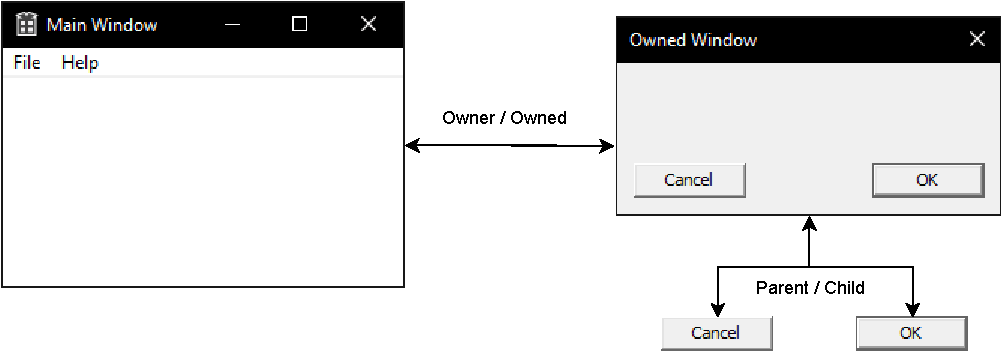
\includegraphics[width=\columnwidth]{obrazky-figures/windows_rels.pdf}
	\caption{Example of owner/owned and parent/child relationships between windows.}
	\label{windowsExample}
\end{figure}

\subsection*{Object handles}
\label{ch2handle}
In Windows, there is no direct access to system resources like files, threads, windows, or graphic images like icons. These system resources are called objects and are unrelated to the C++ object-oriented implementation of objects. For an application to be able to access an object, it needs to obtain an object \textit{handle}.

A \textit{handle} is an opaque data type to access a system resource via the usage of related Windows API functions, which require an object's handle to identify the said object. The value has no real meaning outside of Windows operating system. One can imagine it as an entry of an internal Windows object table. An application can obtain a handle through various Windows API functions, depending on the object the application is trying to access, i.e., using the \lstinline{CreateFile}\footnote{\url{https://docs.microsoft.com/en-us/windows/win32/api/fileapi/nf-fileapi-createfilew}} function to access a file, which returns a handle on success.\cite{HandlesAndObjects}

Handles are kept and managed internally. Depending on the object, a single object can have either multiple handles or be limited to a single handle at a time with exclusive access.\cite{WinHandleLimits}

\subsection*{Function results}
For functions, which return handles, it is easy to tell whether or not the function succeeded at its job. Check whether or not the returned handle is invalid. On the other side, a bunch of lower-level Windows API functions returns \textit{NTSTATUS} as a result.

NTSTATUS is a 32-bit unsigned integer value, which is the result error code of an operation, i.e., a Windows API call. This means that, in general, the value of zero means success, and anything above zero is an error code, holding information about what operation failed. This has an exception, where the values \lstinline{0 - 0x3FFFFFFF} define the success status type, and values 
\lstinline{0x40000000 - 0x7FFFFFFF} define an information status type. This is easily checked with the \lstinline{NT_SUCCESS(x)} macro, where \lstinline{x} is NTSTATUS.\cite{WinNTSTATUS}\cite{WinNTSuccess}

\subsection*{Registry}
The Windows registry is a hierarchical database containing data critical for the Windows operating system's operation, services, and applications that run on it. Data is structure is essentially in a tree format, where the nodes are called \textit{keys}. A key can contain other keys - \textit{subkeys} and entires of data - \textit{values}. 

Registry values have a name, type, and value. Value types are mostly standard Windows types (\ref{winIntegers}) like a double-word, a zero-terminated string, or a generic binary value. There are several predefined (root) keys, each serving a different purpose either for the operating system itself, services, applications, or classes. The root keys are always open and are noted by the \lstinline{HKEY_} prefix.

\begin{figure}[htb!]
	\centering
	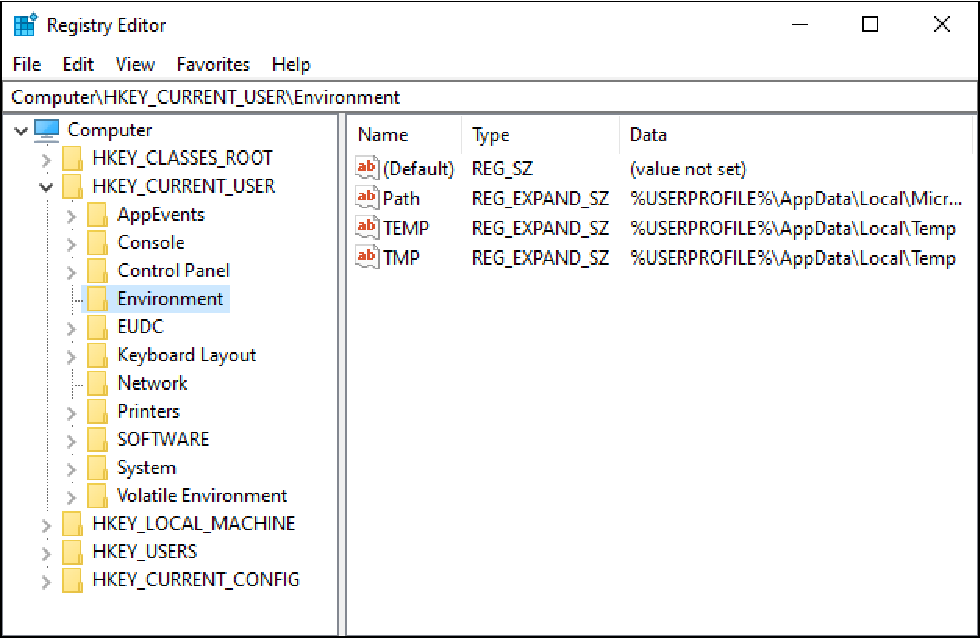
\includegraphics[]{obrazky-figures/regedit.pdf}
	\caption{Browsing Windows registry using the Registry Editor.}
	\label{winRegedit}
\end{figure}

To access a value of a key, one must know its path. The path is a string consisting of all the keys and subkeys, ranging from the root to the leaf key, divided by the backslash character.\cite{WinRegStruct}
For example, in Figure \ref{winRegedit}, to access a value inside the \lstinline{Environment} subkey, the path would be \lstinline{HKEY_CURRENT_USER\\Environment}. The Windows API provides macros for root key specification, which would allow the programmer to emit the specified root key from the path.

For an application, the registry can save user preferences, various settings, remember selected options, or track the application's usage. It is also useful to make the application run automatically upon startup, as implemented in section \todo{autorun}.

\subsection*{Thread synchronization}
There are many ways to synchronize threads in Windows. These include, but are not limited to: Events, Semaphores, Mutexes, Interlocked API, and Slim reader/writer locks (SRW Locks). As this project makes use of SRW locks, this subsection will explain only those in the following.\cite{WinSyncFuncs}

An SRW lock is a simplified version of a semaphore, a synchronization object which is useful in controlling a shared resource between multiple threads. A semaphore has a set number of threads that are allowed to access the resource simultaneously. When a thread is done with using the resource, another thread is allowed to use it.\cite{WinSemaphores} An SRW lock takes the thread's intent with the shared resource into account and is optimized for speed and performance. If a thread wants to read a resource, it can lock the resource in a \textit{shared mode}. If a thread wants to write to a resource, it can lock the resource in the \textit{exclusive mode}. If a resource is not locked, it can be locked in either mode. 

The exclusive mode works just like a semaphore with a single allowed thread. The access is always exclusive as no other threads can simultaneously access the resource, even if some threads only want to read the resource.
The shared mode allows for read-only access to the resource by multiple threads if the lock is not locked in exclusive mode.

Neither mode has a priority of acquiring the lock, there is no order or a queue of access, so if two threads want to lock an SRW lock, it is not predictable which thread will acquire the lock in different modes. An SRW lock is the size of a pointer, which means faster access and a limited amount of information stored about the lock. It is a good, simple choice for a project like this, and is even sufficient enough to solve \textit{"The Readers-Writers Problem}\footnote{\url{https://www.u-aizu.ac.jp/~yliu/teaching/os/lec07.html}}.
\cite{WinSRW}

\section{Microsoft Foundation Class Library}
This section introduces the Microsoft Foundation Class Library (MFC) and aims to provide an overview of important designing functions, implementing the user interfaces.

MFC is a wide-ranged object-oriented C++ library, which abstracts and wraps much of the non-object-oriented Windows API. It is useful for designing and creating user interfaces, small or large dialog boxes, windows, implementing network services, network communication, threading, and more.\cite{MFCDesktop}

\subsection*{Relations to Windows API}
As mentioned in previous sections, MFC allows for much easier desktop application development by abstracting and wrapping a lot of the Windows API, originally only written in C, into the object-oriented C++ programming language.

\begin{lstlisting}[caption={Showing a window using Windows API and MFC}, label=showWindowEx]
//Windows API - Using C
HWND hMainWnd = CreateWindowW(...);
ShowWindow(hMainWnd, SW_SHOWNORMAL);

//MFC - Using C++
AfxGetMainWnd()->ShowWindow(SW_SHOWNORMAL);
\end{lstlisting}

Listing \ref{showWindowEx} showcases an example of showing the main window (\ref{ch2Windows}) using both APIs and an instance of abstracting the window handle away in favor of using a window C++ object. Calling the \lstinline{ShowWindow}\footnote{\url{https://docs.microsoft.com/en-us/windows/win32/api/winuser/nf-winuser-showwindow}} function directly from a window object is a lot more straightforward and convenient than handles. However, it is important to keep in mind that MFC still internally uses the Windows API.
This means, if there is a need for a handle of an MFC object, there are supportive functions like \lstinline{GetSafeHwnd}\footnote{\url{https://docs.microsoft.com/en-us/cpp/mfc/reference/cwnd-class?view=msvc-160##getsafehwnd}}, which return the internal object handle.

\subsection*{Coding conventions}
In MFC, all global static functions are marked with an \lstinline{Afx}, prefix (Application Framework Extension).

\subsection*{Wrappers}

\subsection*{Strings}

\subsection*{Exception handling}

\todo{Overview key MFC parts for this project}

%=============================================================================================================================
\chapter{Virtual File System technologies}
\label{ch3}
This chapter serves as an overview of available virtual filesystem technologies that would allow for direct integration with the Windows desktop environment. Such an instance of virtual filesystem implementation is a Filesystem in userspace (FUSE), "a filesystem in which an ordinary userspace process provides data and metadata".\cite{FUSE}

This exact implementation does not exist on Windows without a kernel-mode driver\cite{WinKernelFS}. Since creating a kernel-mode driver is out of this thesis's scope, the details of how this can be implemented using a third-party virtual filesystem software are shown in section \ref{vfsapitypes}.

The following sections contain the introduction to files, filesystems, and an overview of available third-party APIs that can be considered a valid virtual file system sofware option for this project's intent.

\section{Introduction to filesystems}
The following section helps to understand what a file system is, which operations are the file system's responsibility, how it talks to the file system, how it is defined on a typical file system.

\subsection*{File}
\label{file}
Generally, in Windows, a \textit{file} is a unit of data in a filesystem. A file is stored on a storage device\footnote{i.e. Hard Drive} and consists of one or multiple streams of bytes, which hold related data, and a set of attributes that describe the file and its data. The filesystem manages it, and any application that wants to access, read, write, or execute a file or its attributes has to interact with its respectable filesystem to do so. A file must follow the filesystems' rules, i.e., a file must have a unique name in its directory in NTFS\footnote{New Technology File System}.\cite{FilesAndClusters}

Files in Windows are never accessed directly. Instead, applications on Windows can access a file through its handle (Section \ref{ch2handle}). When a file is opened, a handle is associated with it until the requesting process terminates or the handle is closed. Each handle is unique to each process that opens a file, and depending on which type of access to the file was requested, if one process holds a handle to a file, a second process trying to open a handle to the same file might fail.\cite{FileHandles}

\subsection*{Filesystem}
A filesystem is a process that describes where and how files are stored on a storage device. It allows applications running on the system to access, read and store files. All Windows supported file systems have the following storage components:\cite{LocalFileSystems}

\begin{itemize}
    \item \textbf{Volumes}
    \item \textbf{Directories}
    \item \textbf{Files}
\end{itemize}

A Volume is a place where the filesystem resides, is the highest level of organization in a filesystem, and has at least one partition, a logical division of a physical disk.\cite{WinVolumeMgmt} For this project's purposes, only volumes with a single partition (simple volumes) will be considered. Such volume can be called a \textit{drive} if it is recognizable and accessible by its assigned \textit{drive letter}. 
A drive letter is a single capitalized letter of the alphabet ranging from A to Z, meaning Windows only supports a maximum of 26 drives with drive letters at the same time. For simplicity, the process of assigning a volume to a drive letter while making it accessible in the system will be referred to as \textit{mounting} the volume (The system can mount volumes to directories as well).

A directory is a hierarchical collection of files, can itself be organized into a directory, and has no limitations on the number or capacity of files that it contains. The only limit is defined by the filesystem itself and the capacity of the storage device.\cite{WinDirectoryMgmt} Its important to remember that inside the Windows API a directory can be referred to as a file with a special flag \lstinline{FILE_BACKUP_SEMANTICS}.

A file (\ref{file}) is the related data, and it can be organized into a directory or reside directly in the root of a volume.

\subsection*{File path formats}
Windows uses the standard, traditional DOS\footnote{Disk Operating System} path format, which consists of the following components:

\begin{itemize}
    \item \textit{A volume or drive letter} - It is expected to be followed by the volume separator character\footnote{The colon character (:)}
    \item \textit{A directory name} - The directory separator character\footnote{The backslash character (\textbackslash{})} separates subdirectories within the hierarchy
    \item \textit{An optional filename} - The directory separator character separates the file path and the filename
\end{itemize}

If all three components are present, the path is called an \textit{absolute} path. If no volume is specified and the path begins with the directory separator character, the path is relative from the current drive's root. Otherwise, it is relative to the current directory.\cite{WinPathFormats}

\begin{table}[!hbt]
\centering
\caption{Examples of valid file paths}
\label{filepathsex}
\begin{tabular}{|l|l|l|l|}
\hline
\textbf{Path} & \textbf{Description} \\ \hline
C:\textbackslash{}dir\textbackslash{}test.pdf       & Absolute path from the root of drive \textit{C}    \\ \hline
\textbackslash{}dir\textbackslash{}test.pdf      & Relative path from the root of current drive     \\ \hline
test.pdf       & Relative path from the current directory     \\ \hline
\end{tabular}
\end{table}

\section{Virtual Filesystems}
\label{vfs}
A virtual filesystem is an abstraction of a regular file system - any information, any data, can be organized and presented as a file system. It does not require a storage device to reside on, as it can use one of the existing ones and reside and extend upon it. It can set its own rules on volume, directory, and file management and enforce them. A virtual filesystem's power also comes from integrating closely with the Windows operating system - hooking into the system's internal file operations and handling them in its own way.

To achieve this, this project uses a third-party virtual filesystem software, which exposes a virtual filesystem API. In general, such an API usually allows to create a virtual filesystem by providing the programmer with a list of file operation functions that he must implement. These usually consist of functions that handle creating files, deleting files, reading files, etc. Once these functions are implemented, the user-mode library used to implement them provides them to the kernel-mode driver, allowing this new filesystem to be recognized by Windows. The process of calling implemented file operations works in reverse order. For example, when opening a file, the Windows I/O\footnote{Input\textbackslash{}Output} subsystem, which runs in kernel-mode, forwards this information to the filesystem driver, which can then invoke user-implemented functions request and handle the file operation (open the file).\cite{GitDokany}

This means that a virtual filesystem has to implement all the Windows operating system's important file operations to be functional. Upon implementing, a filesystem can even be shown directly in the Windows Explorer, and be accessibile to all running programs if the virtual drive of the filesystem is mounted. This is usually done internally within the third-party API. The following subsection covers some of the popular options of virtual filesystem software.

\subsection*{Virtual filesystem software}
\label{vfsapitypes}
In general, there two ways a virtual filesystem software can implement a virtual filesystem API:

\begin{itemize}
    \item Native API
    \item FUSE Compatibile API
\end{itemize}

A \textit{Native API} aims to be as close to the intended system it interfaces with as possible, without potentially harmful compromises at the cost of cross-platform compatibility or other factors unrelated to the system. This type can potentially be lower-level than FUSE API and must be well documented by its provider to be usable. As noted by its name, tying closely to a single system means the API focuses on working on the intended system as seamlessly as possible. For windows specifically, native API requires two components, a kernel-mode driver and a user-mode library which interacts with it.

\begin{itemize}
    \item \textit{Pros}: Good optimization, coding constructs similiar to the targeted system, all features of the targeted system
    \item \textit{Cons}: Little to no cross-platform compatibility, lower-level API requires deeper knowledge of the targeted system, steeper learning curve
\end{itemize}

The \textit{FUSE Compatible API} is meant to be compatibile with FUSE, a high-level API originally only for Linux. Compatibility with FUSE allows for cross-platform compatibility with little to no changes to the implementation of the virtual filesystem. For Windows specifically, the implementation of filesystems is vastly different from Linux, and usage of a FUSE compatibile API comes with its compromises, such as lower performance, or excluding some of the features only present in Windows, i.e., volume labels.\cite{WinFspVSFUSE}\cite{FUSE}

\begin{itemize}
    \item \textit{Pros}: Cross-platform compatibility, easier development with higher-level API, well documented API
    \item \textit{Cons}: Lack of Windows specific features, restricted by POSIX standards
\end{itemize}

For this thesis, it is much preferable to choose a API software option which includes a native API, as cross-platform compatibility is not a requirement, and thus, there is no need for any restrictions. Additionally, being able to use Windows specific filesystem related features is a step towards better user experience. An open-source licence of the software would also be preferred.

\subsection*{Dokany}
Dokany is one of the oldest, yet still fully functional pieces of virtual filesystem software. It was created in 2007 and while undergoing a switching of its developers, it is still being developed today.

\begin{itemize}
    \item \textit{Supported API types}: Native, FUSE wrapper
    \item \textit{Supported languages}: C (default), Java, Delphi, DotNet, Ruby
    \item \textit{Supported architectures}: x86, x64, ARM, ARM64
    \item \textit{Suppored desktop operating systems}: Windows 7 SP1 / 8 / 8.1 / 10
    \item \textit{Open-source}: Yes
    \item \textit{Provides a driver}: Yes
\end{itemize}

In conclusion, Dokany is a well supported, stable piece of software, nearly an ideal choice for projects which pay excessive attention to software stability and compatibility, while being able to create a filesystem in various, even higher-level programming languages, rather than just the low-level C.\cite{GitDokany}\cite{DokanDevIo}

\subsection*{VFSForGit}
Virtual File System for Git is software, developed by Microsoft to enable Git\footnote{\url{https://git-scm.com/}} at a high level, enterprise, scale. VFSForGit virtualizes a Git repository into a virtual filesystem, this is a form of integrating the files, which are not physically present on the users computer, rather still being present on the Git repository while being displayed. The contents of the files can be downloaded on request. 

\begin{itemize}
    \item \textit{Supported API types}: Native GVFS Protocol\footnote{\url{https://github.com/microsoft/VFSForGit/blob/master/Protocol.md}}
    \item \textit{Supported languages}: Git commands
    \item \textit{Supported architectures}: x64
    \item \textit{Suppored desktop operating systems}: Windows 10 version 1607, or later
    \item \textit{Open-source}: Yes
    \item \textit{Provides a driver}: Yes
\end{itemize}

VFSForGit is a virtual filesystem software aimed towards usage with Git repositories, especially at larger scales. It doesnt provide many languages or options for architectures and only supports newer versions of Windows 10. With those restrictions in mind, it is still being supported and is an useful tool for accessing Git respositories in the Windows environment.\cite{GitVfsForGit}\cite{VfsForGitMS}

\subsection*{WinFsp}
Windows File System Proxy is a performant, stable collection of software components, which allows for implementing a virtual filesystem using one of its supported API layers. The focus of WinFsp is on high compatibility with NTFS, the default filesystem of Windows. This allows for smooth integration with the Windows environment and for virtual fielsystems, which use or extend NTFS.

\begin{itemize}
    \item \textit{Supported API types}: Native, FUSE compatibility layer
    \item \textit{Supported languages}: C, C++, DotNet
    \item \textit{Supported architectures}: x86, x64, ARM, ARM64
    \item \textit{Suppored desktop operating systems}: Windows 7 and above
    \item \textit{Open-source}: Yes
    \item \textit{Provides a driver}: Yes
\end{itemize}

WinFsp is a great option for any virtual filesystem implementation, which will be running only on Windows. Whether its one of the older versions of the operating system, or the newer one, WinFsp provides continuous support and compatibility with those systems, while keeping the officialy supported langues of its API layers both lower and higher level, thanks to inclusion of C++ and DotNet. Its a great choice for any project starting from scratch, or from a project that was originally built for FUSE.\cite{GitWinFsp}

\section{Windows File System Proxy}

The third-party filesystem software of choice of this project is Windows File System Proxy (WinFsp). VFSforGit could not be used, because of its limitations and focus on Git repositories, since the VDU project does not expose any Git respositories. This is further mentioned during analysis in chapter \ref{ch4}. Dokany was a great option, stable, supported, and similiar with compatibility layers to WinFsp. On the other hand, WinFsp has a native API support for C++, which allows for cleaner and easier to understand code, and offers much better performance and optimization than Dokany. This is proven by various filesystem operation tests done to compare versions of WinFsp against Dokany and NTFS. These charts can be seen in figures \ref{winfsp_file_tests} and \ref{winfsp_rdwr_tests}.

\begin{figure}[htb]
	\centering
	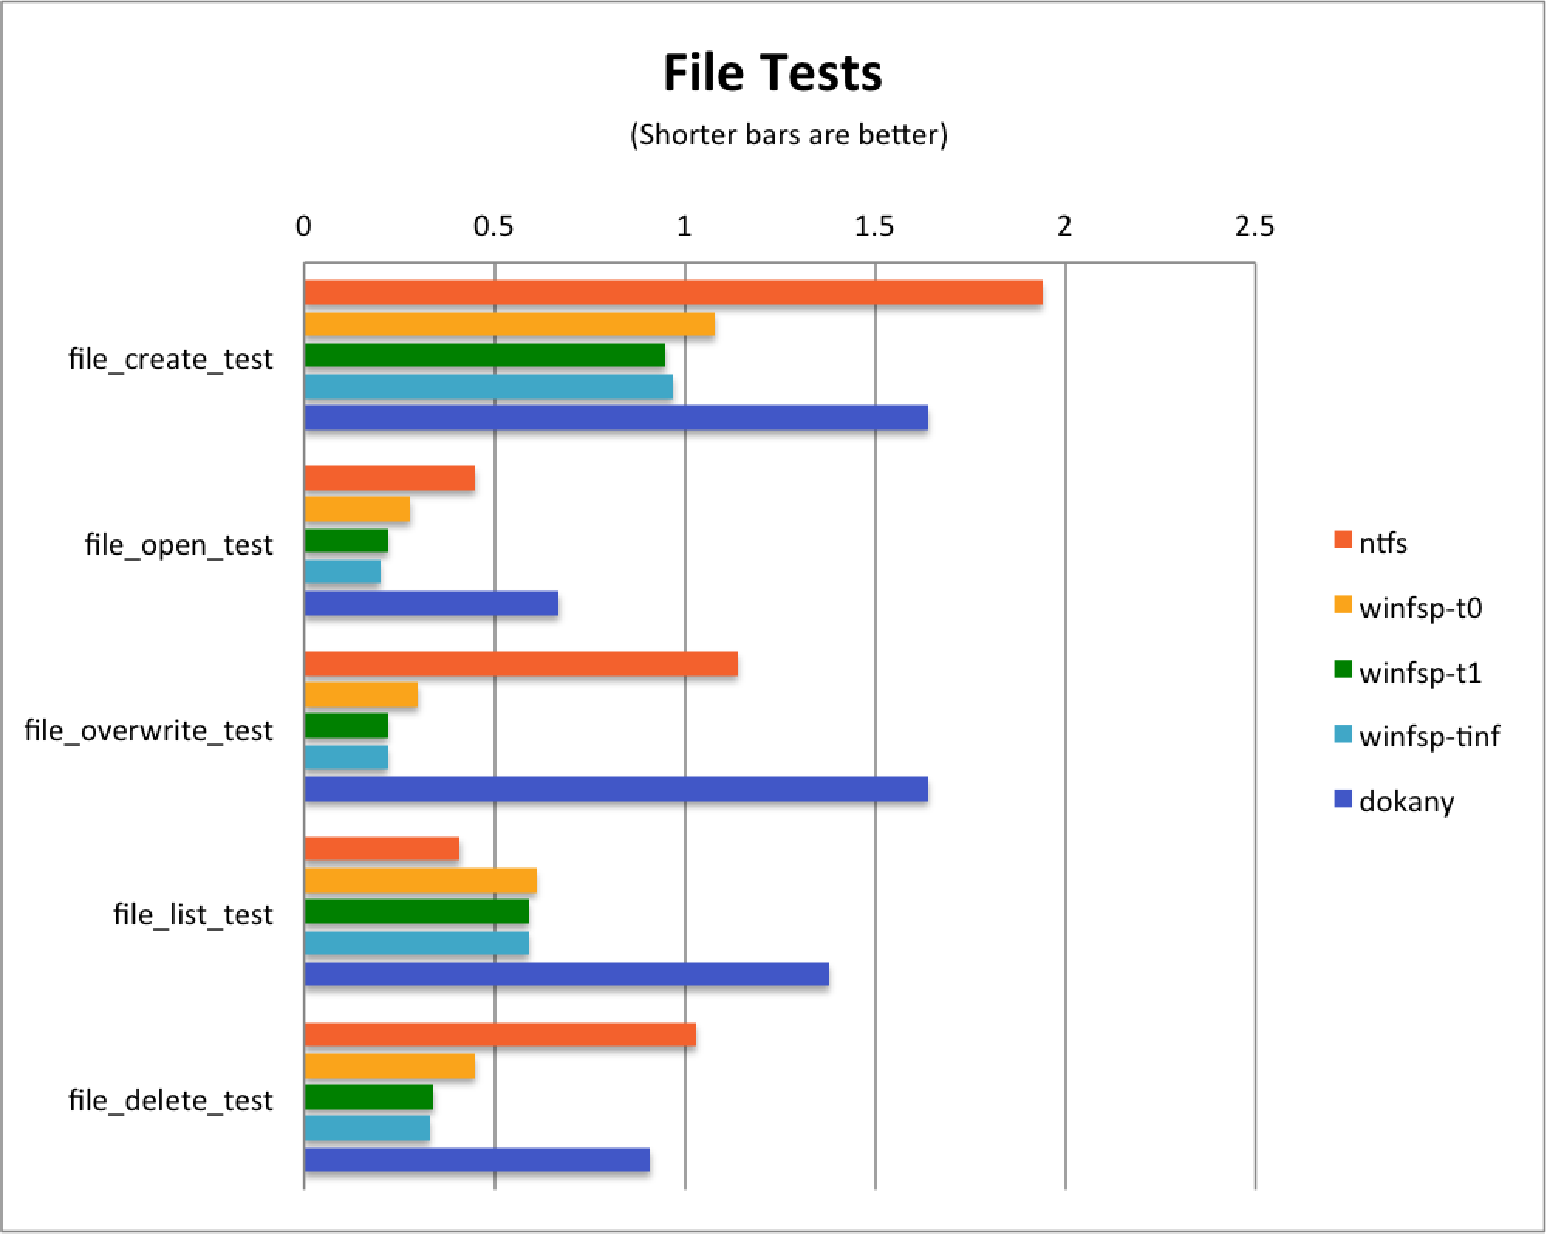
\includegraphics[width=\columnwidth]{obrazky-figures/file_tests.pdf}
	\caption{File comparation tests of WinFsp and Dokany. Source:\cite{GitWinFsp}}
	\label{winfsp_file_tests}
\end{figure}

\begin{figure}[htb]
	\centering
	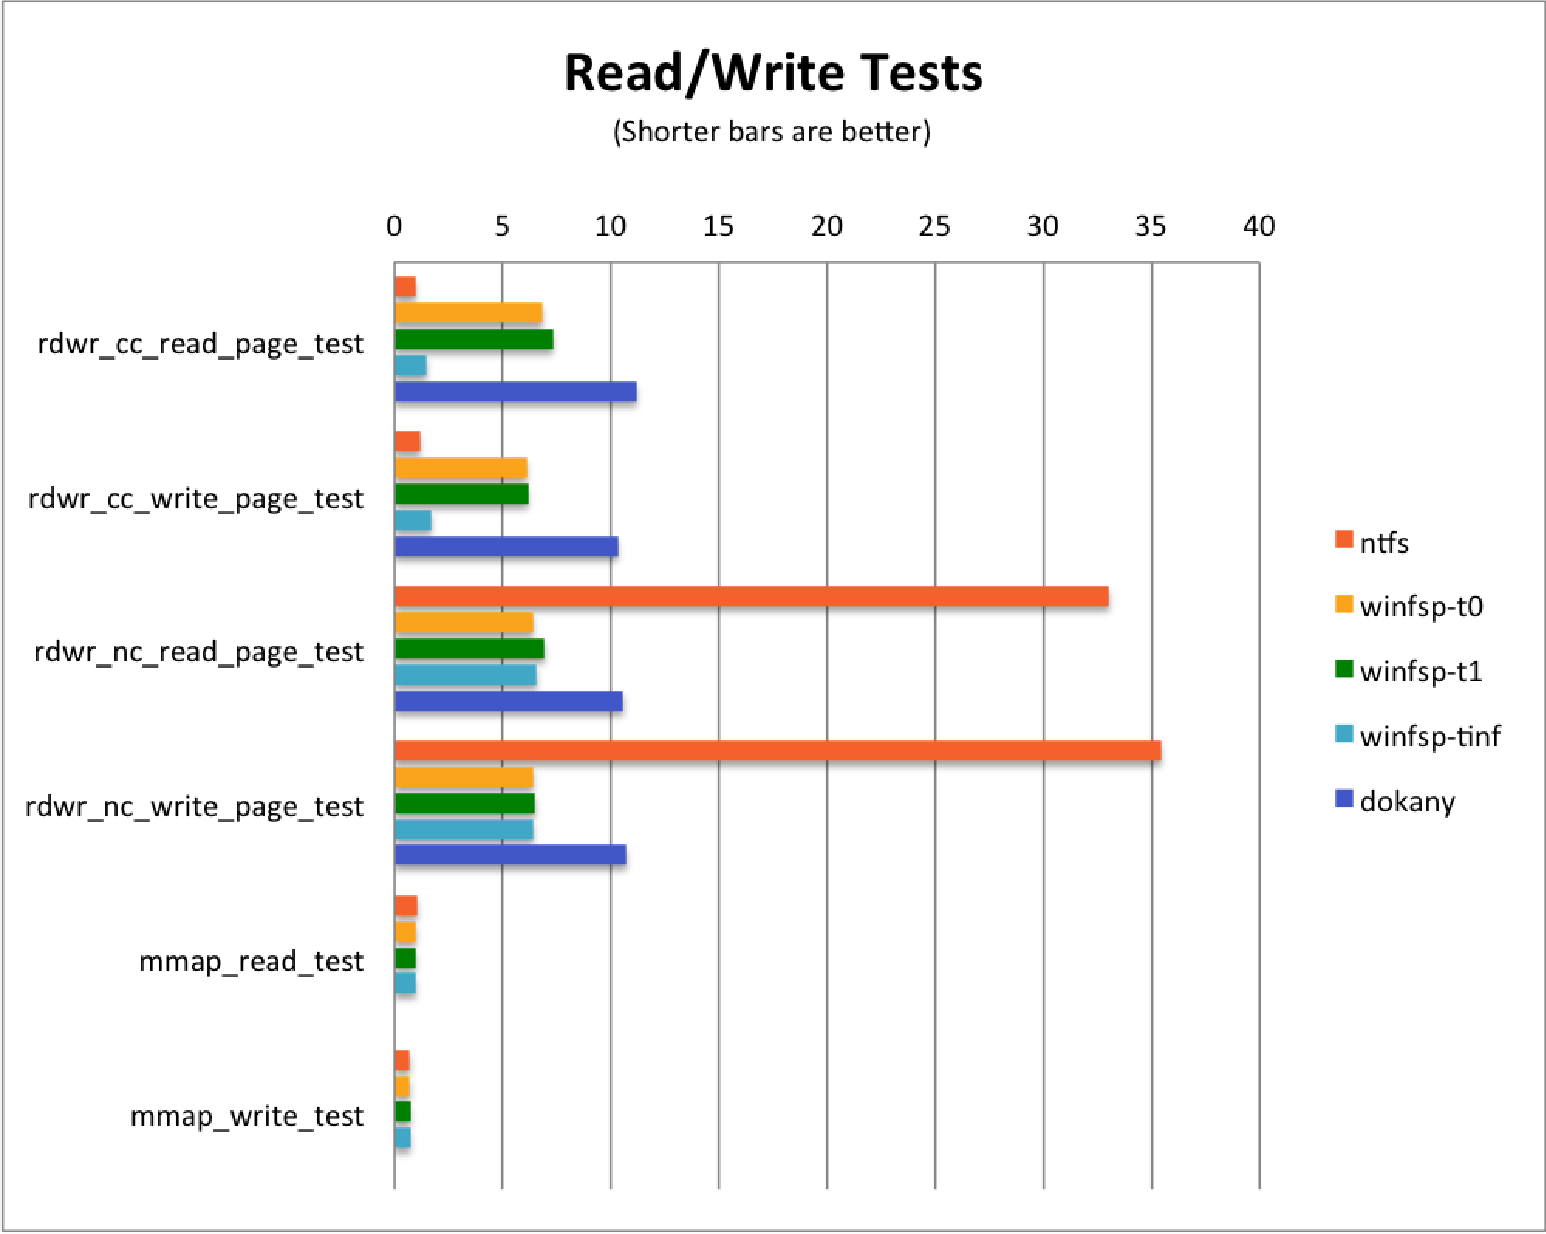
\includegraphics[width=\columnwidth]{obrazky-figures/rdwr_tests.pdf}
	\caption{Read and write comparation tests of WinFsp and Dokany. Source:\cite{GitWinFsp}}
	\label{winfsp_rdwr_tests}
\end{figure}

\newpage
\subsection*{Introduction}
WinFsp is
\todo{Introduce winfsp}

%=============================================================================================================================
\chapter{Analysis}
\label{ch4}
%=============================================================================================================================
This chapter will tackle the first step of creating an application, the analysis, and steps taken during an analysis of provided documentation. It will introduce required technologies to understand and handle them. Results of the analysis are present at the end of this chapter.

\todo{Include google docs pdf of requirements?}

\section{Required technologies}
In this project, the provided documentation was received as a non-formal description of the server's REST API the client is supposed to be accessing. As this documentation is written in plain text, it requires proper analysis, understanding of the underlying technologies, and formalization into a better format. This section serves as an overview of these technologies.

\subsection*{Hypertext Transfer Protocol}
The Hypertext Transfer Protocol (HTTP) 

\cite{MozillaHTTP}

\subsection*{Representational State Transfer API}
The Representational State Transfer (REST) represents an architectural style for distributed multimedia systems. It's a programming style for developing RESTful web services, which allows the developer to take advantage of an existing protocol, HTTP. It conforms at the very least to the most basic REST constraints, as defined by its creator \textit{Roy Thomas Fielding}:

\begin{itemize}
    \item \textit{Client-Server} - Separates the client's side and the server's side
    \item \textit{Stateless} - Each request must contain all necessary information necessary to understand the request
    \item \textit{Cache} - Requests must be labeled as cacheable or non-cacheable. Improves network efficiency if it is available
\end{itemize}

These constraints are further extended specifically to address web services:
\begin{itemize}
    \item \textit{Uniform Interface} - Increases scalability at the cost of effectivity, uses a single standardized form
    \item \textit{Layered System} - Architecture composed of hierarchical layers, each component can not access other components beyond the immediate layer with which it is interacting
    \item \textit{Code-On-Demand} - Allows client functionality to be extended by downloading and executing code in the form of applets or scripts to improve system extensibility
\end{itemize}

The key abstraction of information in REST is a \textit{resource}. A resource can be anything that can be named and might be a potential target of a request, e.g., a document, an image, a data file. Interactions, i.e., manipulating a resource, happen between two parties, as noted by the first constraint, the client and server. If a client requests an operation with a resource, it sends an HTTP request, where the HTTP method is the type of operation, and the HTTP object path is the path to the resource. After processing the request, the server can inform the client about the operation's state via the HTTP status code in the HTTP response.\cite{RestAPI}

\begin{table}[hbt]
\centering
\caption{Examples of REST API requests}
\label{restapiex}
\begin{tabular}{|l|l|l|l|}
\hline
\textbf{Method} & \textbf{Path} & \textbf{Description} \\ \hline
 GET & /users & Get all users \\ \hline
 POST & /users/john & Update an user  \\ \hline
 DELETE & /users/john &  Delete an user \\ \hline
 PUT & /users & Add an user \\ \hline
\end{tabular}
\end{table} 

\subsection*{OpenAPI}
The OpenAPI Specfication is an API description format for REST APIs. An entire API can be described with just a single file of the OpenAPI format, which supports file formats of either YAML\footnote{A recursive acronym for "YAML Ain't Markup Language"} or JSON\footnote{JavaScript Object Notation}. OpenAPI describes:

\begin{itemize}
    \item Available endpoints and operations on each endpoint
    \item Operation parameters, and input/output for each operation
    \item Authentication methods
    \item Contact information, terms of use, other information
\end{itemize}

The OpenAPI format is easily readable by both machines and humans. Many third or first-party services provide a way to visualize the API in a graphical format, i.e., the Swagger Editor\footnote{\url{https://editor.swagger.io/}}.\cite{SwaggerDocs}

\newpage
\begin{lstlisting}[caption={An example of an OpenAPI file in the YAML format}, label=openapiex]
#A simple documentation of a /ping endpoint
openapi: 3.0.0 
info:
  version: '1.0' 
  title: An amazing API
  description: A formal description
servers: #Server URL for testing
  - url: 'https://localhost:4443'
paths: #Endpoint descriptions
  /ping: #Endpoint path
    get: #Method
      parameters: [] #Call parameters
      description: To test a connection.
      responses: #Possible responses
        '204':
          description: Ping success!
\end{lstlisting}

\todo{More about openapi, like, basic structure? Probably not necessary tho.}

\section{Formalization}
In the context of provided documentation, formalization means creating an OpenAPI specification based on the documentation's plain text version. A formalized specification allows for better readability, understanding, development, and testing on the developer's side. The formalized specification's concrete usage is covered in chapter \ref{ch6}, implementing the client, and \ref{ch7} for implementing and testing a mock server.

\subsection*{Creating the specification}
Formalizing the provided documentation consists of reading and understanding all the API endpoints and their access or usage restrictions and manually creating an entry for each one in an OpenAPI file. Each entry has its own possible status codes, headers, and content, which endpoint could return. For this project, I used the Swagger Editor, which allowed me to document the VDU API more comfortably. The editor's great advantage is that it can render the OpenAPI specification file in an HTML\footnote{Hyper-Text Markup Language} 5 format, as shown in figure \ref{swagger_result}.

\begin{figure}[htb]
	\centering
	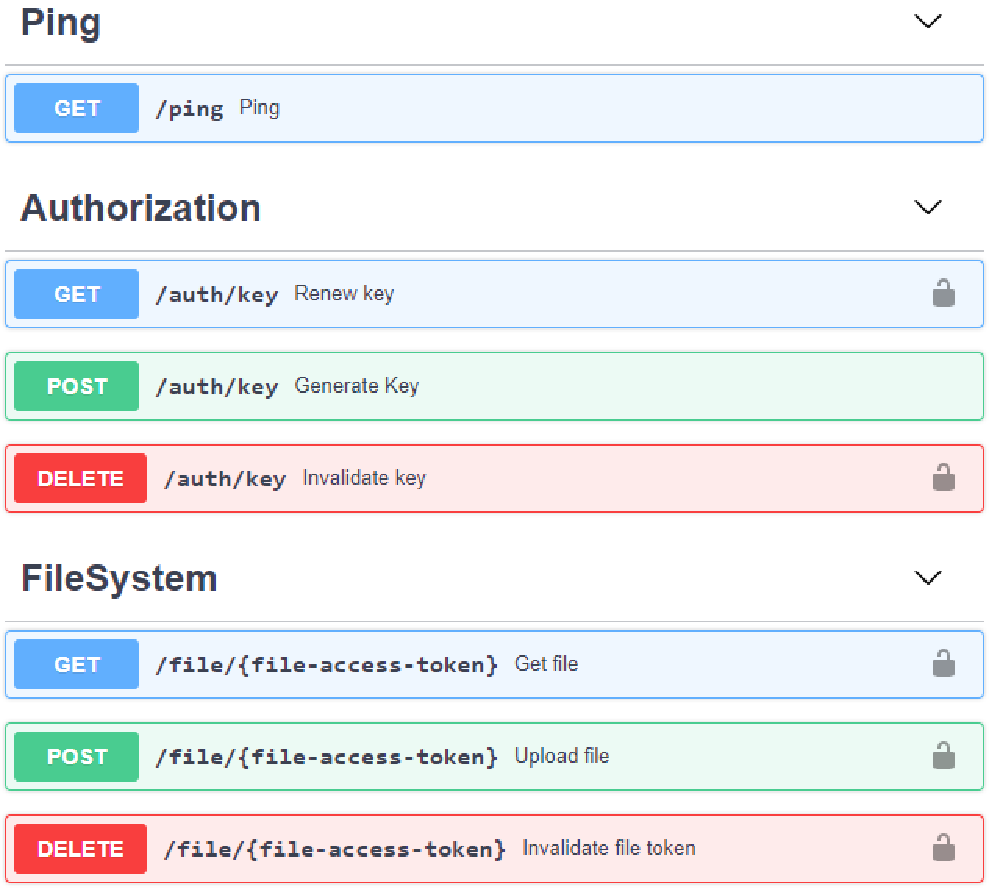
\includegraphics[width=\columnwidth]{obrazky-figures/swagger_result.pdf}
	\caption{VDU REST OpenAPI 3.0 summary, rendered using the Swagger Editor, authentication requirement is signified by the lock icon.}
	\label{swagger_result}
\end{figure}

I analyzed and noted all the API access requirements, each method, its parameters, return values, and how they tie to each other from the formal, well-specified API documentation. Afterward, I discussed this information further with my supervisor, which allowed me to understand better how the API works and how it should interact.

\section{Results}
This section will summarize the result of the VDU API documentation analysis. These results are used to guide the design of the application in Chapter \ref{ch5}.

\subsection*{Endpoints}
This section lists all available VDU API endpoints, as shown in figure \ref{swagger_result} and provides an overview of their usages. Some endpoints require an \textit{X-Api-Key} (API key) for successful access.

\begin{itemize}
    \item \textit{GET} \textit{/ping} - Tests a connection to the server
    \item \textit{POST} \textit{/auth/key} - Authenticates an user by name or email. Client secret can be included in the content if necessary. Returns API key on success.
    \item \textit{GET} \textit{/auth/key} - Returns a new API key with new expiration time, refreshes session
    \item \textit{DELETE} \textit{/auth/key} - Invalidates API key
    \item \textit{GET} \textit{/file/\{file-access-token\}} - Returns file contents, additional file information is in the response headers
    \item \textit{POST} \textit{/file/\{file-access-token\}} - Uploads file contents, additional file information has to be in the request headers
    \item \textit{DELETE} \textit{/file/\{file-access-token\}} - Invalidates a file token, does NOT delete the file from VDU system
\end{itemize}

\subsection*{Access}
Both client and server must use a secure TLS\footnote{Transport Layer Security} channel to access the VDU API, while the server must have a valid server-side TLS certificate. This implies the usage of HTTPS protocol to access the API. The client-side certificate is optional and allows the user to omit the client secret from the authentication endpoint.

The authentication is done using an API key, which is at first obtained from the \lstinline{POST /auth/key} endpoint. An API key has its expiration date, which a client must respect, and the key has to be refreshed using the \lstinline{GET /auth/key} endpoint if it is about to expire. The client can prematurely invalidate the API key with the \lstinline{DELETE /auth/key} endpoint.

File tokens, seen as \textit{\{file-access-token\}} in the \lstinline{/file/} endpoint path, are generated from the proprietary VDU web user interface. Each token represents a single file, has an expiration date, and can be prematurely invalidated using the \lstinline{DELETE /file/} endpoint. This file can be modified using the \lstinline{POST /file/} endpoint, which includes modifying its content and file name. A file can be read-only, meaning that the server will deny any modification request.


%=============================================================================================================================
\chapter{Design}
\label{ch5}
%=============================================================================================================================
This chapter aims to design the application based on knowledge from previous chapters. The designing processs consists of two main parts - the visual and the inner application design part. The visual part takes care of the user interface, user experience, all the windows, menus, buttons and overall feeling of the application for the user. The inner application part revolves around the class structure and relationships, chooses coding practices and various internal options for designing the application, which are implemented in chapter \ref{ch6}.

\section{User interface}

\begin{figure}[htb]
    \centering
    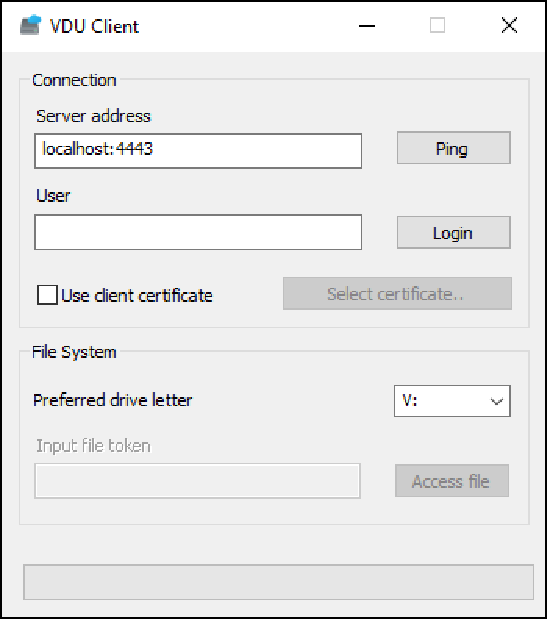
\includegraphics[]{obrazky-figures/clientui.pdf}
	\caption{User interface of the VDU Client application.}
	\label{clientui}
\end{figure}

\begin{figure}[htb]
    \centering
    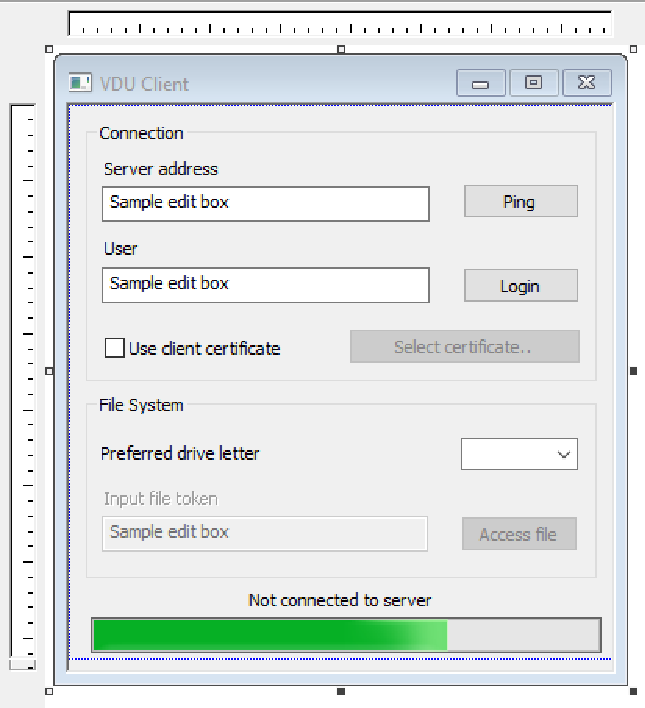
\includegraphics[]{obrazky-figures/resourceeditorui.pdf}
	\caption{User interface of the VDU Client application, designed in the Visual Studio resource editor.}
	\label{resourceeditorui}
\end{figure}

\section{Coding practises}

\section{Class structure}

\begin{figure}[htb]
	\noindent
	\makebox[\textwidth]{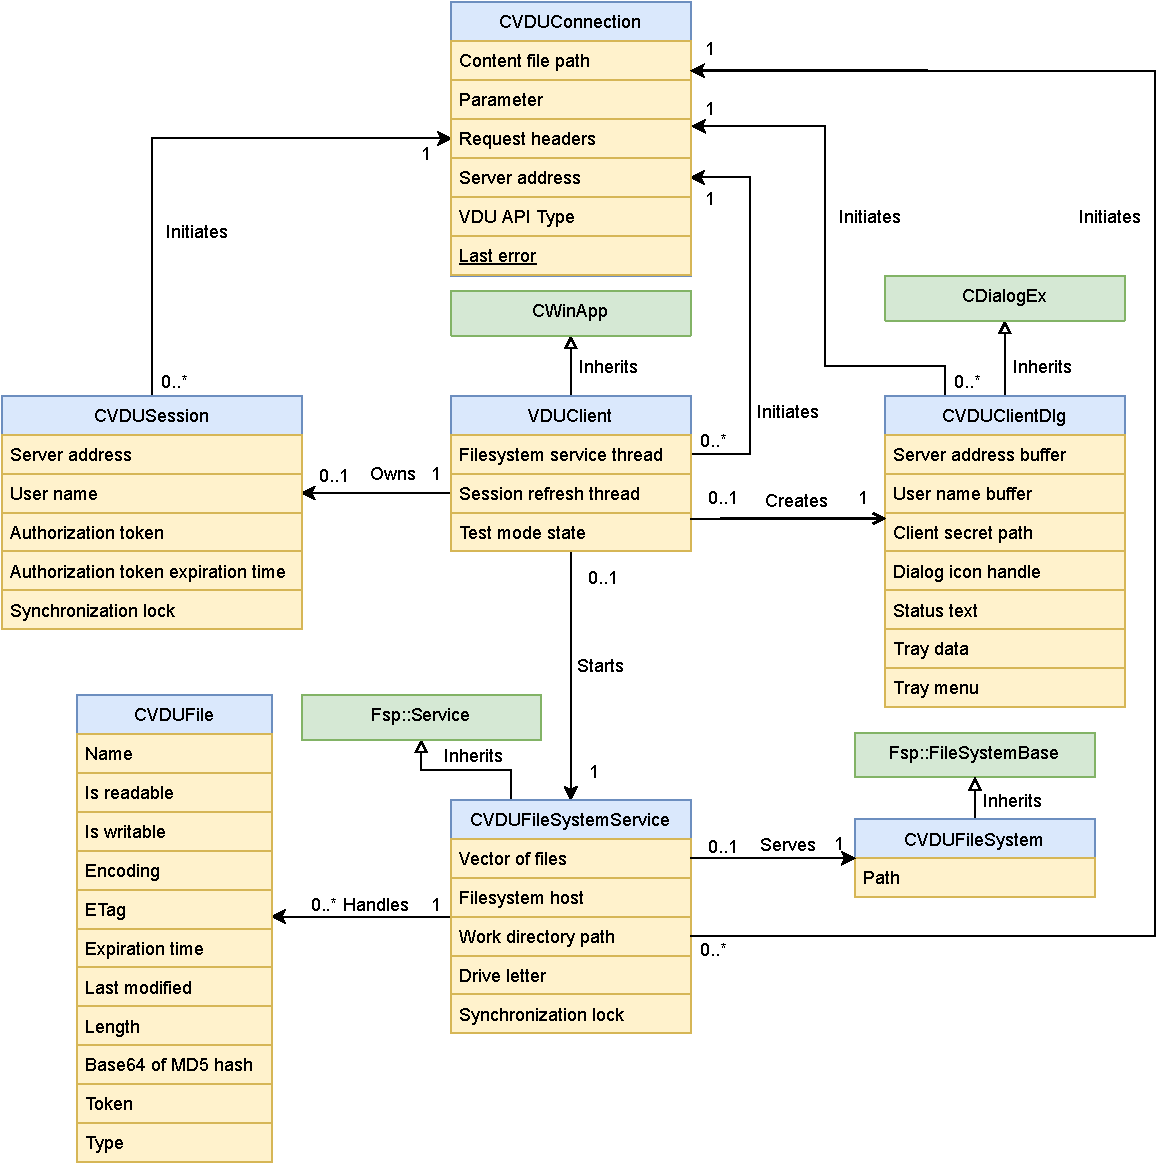
\includegraphics[]{obrazky-figures/vduclassdiagram.pdf}}
	\caption{Class diagram of the VDU Client application.}
	\label{vduclassdiagram}
\end{figure}

%=============================================================================================================================
\chapter{Implementation}
\label{ch6}
%=============================================================================================================================
Implementation

\section{User Interface}

\section{Connection}

\section{Thread synchronization}

%=============================================================================================================================
\chapter{Testing and verification}
\label{ch7}
%=============================================================================================================================
Testing

\section{Creating a server}

\section{Unit testing}

\section{Results}


%=============================================================================================================================
\chapter{Conclusion}
\label{ch8}
\todo{Evaluation of progress etc.}

The result application was released, and I published the source code as open-source on GitHub\footnote{\url{https://github.com/}}.

%=============================================================================================================================
 